%% LyX 2.1.4 created this file.  For more info, see http://www.lyx.org/.
%% Do not edit unless you really know what you are doing.
\documentclass[12pt,british,sort&compress]{article}
\usepackage{mathptmx}
\renewcommand{\familydefault}{\rmdefault}
\usepackage[T1]{fontenc}
\usepackage[latin9]{inputenc}
\usepackage{geometry}
%\geometry{verbose,tmargin=2m,bmargin=2m,lmargin=2cm,rmargin=2cm,headheight=2.5cm,headsep=1cm,footskip=1.5cm}
\geometry{verbose,tmargin=2cm,bmargin=2cm,lmargin=2cm,rmargin=2cm,headheight=1.15cm,headsep=1.15cm,footskip=1.25cm}
%\geometry{verbose,tmargin=2cm,bmargin=2cm,lmargin=2cm,rmargin=2cm,headheight=2cm,headsep=2cm,footskip=1.5cm}
\usepackage{refstyle}
\usepackage{float}
\usepackage{rotfloat}
\usepackage{amsmath,amssymb}
\usepackage{graphicx}
\usepackage{esint}
%\usepackage{enumitem}

\usepackage{fancyhdr}
\renewcommand{\headrulewidth}{0pt}
\pagestyle{fancyplain}
\fancyhf{}
\fancyhead[R]{FRIA CALL 2016 - FRIA-B1} %\includegraphics[width=8cm]{img/header.png}}
%\fancyfoot[L]{ Name Firstname - v1.0 \\  Date}}
\fancyfoot[C]{\thepage} %\  / \pageref{LastPage}}

\usepackage{tabto}
%\usepackage{biblatex}
\usepackage[style=nature,sorting=none,maxnames=1,backend=biber,refsection=none]{biblatex}
% % Some field suppression via options
% \ExecuteBibliographyOptions{isbn=false,url=false,doi=false,eprint=false}
\addbibresource{MIS-2015.bib}
\renewcommand*{\bibfont}{\footnotesize}

%%%http://tex.stackexchange.com/questions/124513/compressed-abbreviated-bibliography-biblatex-or-otherwise

\makeatletter
% Some field suppression via options
\ExecuteBibliographyOptions{isbn=false,url=false,doi=false,eprint=true}

% One-paragraph bibliography environment
\defbibenvironment{bibliography}
  {\list
     {\printtext[labelnumberwidth]{%
        \printfield{prefixnumber}%
        {[}\printfield{labelnumber}{]}}%
      \ifentrytype{article}{% Suppress remaining fields/names/lists here
        \clearfield{title}}{}}
     {\setlength{\leftmargin}{0pt}%
      \setlength{\topsep}{0pt}}%
      \renewcommand*{\makelabel}[1]{##1}}
  {\endlist}
  {\mkbibitem}

% \mkbibitem just prints item label and non-breakable space
%\makeatletter
\newcommand{\mkbibitem}{\@itemlabel\addnbspace}
%\makeatother

% Add breakable space between bibliography items
\renewcommand*{\finentrypunct}{\addperiod \\} %\space}

% et al. string upright (nature style applies \mkbibemph)
\renewbibmacro*{name:andothers}{%
  \ifboolexpr{
    test {\ifnumequal{\value{listcount}}{\value{liststop}}}
    and
    test \ifmorenames
  }
    {\ifnumgreater{\value{liststop}}{1}{\finalandcomma}{}%
     \andothersdelim
     \bibstring{andothers}}
    {}}
%%%%%%%%%%%%%%%%%%%%%%%%%%%%%%%%%%%%%


%%%%%%%%%%%%%%%%%%%%%%%%%%%%%% LyX specific LaTeX commands.

\AtBeginDocument{\providecommand\figref[1]{\ref{fig:#1}}}
%% Because html converters don't know tabularnewline
\providecommand{\tabularnewline}{\\}
\RS@ifundefined{subref}
  {\def\RSsubtxt{section~}\newref{sub}{name = \RSsubtxt}}
  {}
\RS@ifundefined{thmref}
  {\def\RSthmtxt{theorem~}\newref{thm}{name = \RSthmtxt}}
  {}
\RS@ifundefined{lemref}
  {\def\RSlemtxt{lemma~}\newref{lem}{name = \RSlemtxt}}
  {}


\@ifundefined{date}{}{\date{}}
%%%%%%%%%%%%%%%%%%%%%%%%%%%%%% User specified LaTeX commands.

\usepackage{hyperref}
\usepackage{xcolor}
\hypersetup{
    colorlinks,
    linkcolor={red!50!black},
    citecolor={blue!50!black},
    urlcolor={blue!80!black}
}


%removes unecessary spaces from bullet listing
\usepackage{enumitem}
\setlist{nolistsep}

%for fitting more citations
\usepackage{multicol}


%\bibliographystyle{unsrt}
%to make separate references
%\usepackage[sectionbib]{chapterbib}
%\usepackage[english]{babel}
%\usepackage{biblatex}
%\usepackage[style=authoryear,backend=biber,refsection=none]{biblatex}
%\bibliography{MIS2015.bib}
%\addbibresource{{/home/atul/SparkleShare/ULB repo/intermediate/furtherScholarship/tex/MIS2015.bib}}
%\addbibresource{{/home/atul/SparkleShare/ULB repo/intermediate/furtherScholarship/tex/MIS2015}}
%\addbibresource{{MIS2015}}
%\addbibresource{{MIS2015.bib}}

\makeatother

\usepackage{babel}
\begin{document}
\pagenumbering{roman}

%\begin{flushright}
%\large{FRIA CALL 2016 - FRIA-B1}
%\par\end{flushright}

\hfill{}%
\begin{tabular}{|l|l|}
\hline 
\multicolumn{1}{|l|}{Full name of the applicant} & \multicolumn{1}{l|}{Atul Singh Arora }\tabularnewline
\hline 
SEMAPHORE Application ID & 29379721\tabularnewline
\hline 
\end{tabular}\hfill{}

\medskip{}


\begin{center}
\huge{SCIENTIFIC SECTION OF THE PROPOSAL}
\par\end{center}

\begin{center}
Main language chosen = English
\par\end{center}

\vfill{}

\begin{center}
\fbox{\begin{minipage}[c][1\totalheight][t]{0.7\textwidth}%
\begin{flushleft}
This part includes the following elements:
\par\end{flushleft}
\begin{enumerate}
\item \begin{flushleft}
Description of the research project 
\par\end{flushleft}
\item \begin{flushleft}
\emph{Activities report on the first year of doctorate (ONLY for 1st
grant - 2nd year applicants){*} }
\par\end{flushleft}
\item \begin{flushleft}
Description of the work environment 
\par\end{flushleft}
\item \begin{flushleft}
Summary of the master\textquoteright s thesis or equivalent 
\par\end{flushleft}
\item \begin{flushleft}
Additional comments (optional) 
\par\end{flushleft}
\item \begin{flushleft}
PhD work calendar per month
\par\end{flushleft}
\end{enumerate}
\begin{flushleft}
\emph{{*} ``1st grant - 2nd year'' applicants have already worked
on a full-time basis for one year or more on the PhD project submitted
to the FRIA.}\\

\par\end{flushleft}

\begin{flushleft}
The FRIA insists on strict compliance of the number of pages allowed
for documents that shall be enclosed with the application form and
stresses again the sovereign consideration of the Juries in case the
file would exceed the applicable page limit.
\par\end{flushleft}%
\end{minipage}}

\end{center}

\vfill{}

\clearpage{}

\pagenumbering{arabic}


\section{DESCRIPTION OF THE RESEARCH PROJECT}

%\begin{refsection}
\newrefsection



\subsection{Goals of the Research}

Current information processing models are fundamentally limited in terms of speed, efficiency, security and privacy, as they assume a simplified representation of the world, relying on classical physics. In the past few decades, research in the field of quantum information processing has been carried out to break this barrier by exploiting quantum phenomena. This has led to breakthrough results such as Bennett and Brassard's informationaly secure quantum key distribution protocol~\cite{BB84} and Shor's efficient factoring algorithm~\cite{shor94} which suggest that future large-scale network of computing devices will be able to communicate both efficiently and securely using quantum resources. 

Despite steady progress, including practical implementations of quantum key distribution schemes, there are both technological limitations and theoretical barriers. The development of algorithms and protocols exploiting such a quantum network to its full capacity is also hindered by the inherent difficulty at characterising interactive quantum communication models. As a consequence, only limited techniques are known for studying quantum communication complexity and the development of fundamental cryptographic primitives, such as quantum coin flipping, requires complicated tools. % that make it extremely hard to derive explicit protocols.

The overall aim of this research project is to take a fresh start towards quantum communication protocols by approaching their theoretical foundations from a new perspective. More precisely, our objectives are the following: 
\begin{enumerate}[
labelindent=*,
style=multiline,
leftmargin=*,
label=\arabic*)
]
\item The development of a new framework to study quantum communication protocols based on continuous-time Hamiltonian evolution. 
\item New techniques to obtain strong lower bounds in quantum communication complexity and matching efficient protocols. 
\item  Practical and optimal quantum protocols for cryptographic primitives, in particular for coin flipping.
 \end{enumerate}

\subsection{State of the Art \label{sub:state-of-the-art}}

\emph{Communication complexity} is a computational model first introduced by Yao~\cite{Yao79} where two distant players, Alice and Bob, each receive an input $x$ and $y$ respectively and their goal is to compute a function $f(x,y)$. To this end, they must communicate and the communication complexity is defined as the minimum number of bits Alice and Bob must exchange in order to compute the function with at most $\epsilon$ error. In addition to being quite a natural computational model on its own, communication complexity has also found many applications, not only for proving bounds via reductions for other computational models (decision trees, streaming algorithms) but also for more practical problems such as the design of VLSI circuits (see, e.g.,~ \cite{KN97}). 

For this reason, communication complexity has been extensively studied, however,  progress has been quite slow due to the difficulty of developing good lower and upper bound techniques. In particular, the famous log-rank conjecture \cite{LS88}, which states that the communication complexity of a function is bounded from above by a constant power
of the rank of its communication matrix $M_{x,y}=f(x,y)$, remains open despite decades of attempts to prove it. 

Over the last few years, a new approach to communication complexity problems based on information theory has attracted a lot of interest. This approach can not only be used to prove lower bounds on the usual model but also leads to a new model called \emph{information complexity}, where the cost of a communication protocol no longer corresponds to the length of the communicated messages but rather to their information content (see, e.g.,~\cite{Bra12}). Information complexity is also equivalent to amortised communication complexity \cite{BW12} and therefore leads to an interactive analogue of Shannon compression. It has recently been shown that some lower bound techniques for communication complexity also lower bound information complexity~\cite{KLL+14}. These techniques draw an interesting connection with the notion of Bell inequalities studied in the context of quantum non-locality, which makes it possible to define natural extensions of these lower bound techniques to \emph{quantum communication complexity}~\cite{LLR12}, an extension of communication complexity where the players can exchange quantum messages. %This line of research is quite promising as the set of lower bound techniques for quantum communication complexity is currently even more limited than for its classical counterpart. 

While the set of lower bound techniques for quantum communication complexity is very limited, closely related computational models are much better understood, such as \emph{quantum query complexity}, the quantum analogue of query complexity or \textquotedblleft decision tree complexity\textquotedblright, which in the bounded-error case is known to be characterised by a semidefinite program called the \emph{adversary bound}~\cite{LMRSS11}. The proof of this fundamental result is facilitated by considering a generalisation of the model where the goal is not to compute a function but rather to generate
a quantum state~\cite{AMRR11}. More recently, an alternative proof was provided by my promoter by considering a continuous-time model of quantum query complexity~\cite{BR14}. 

\emph{Coin flipping} is a fundamental cryptographic primitive where two distrustful parties need to remotely generate a shared unbiased random bit. A cheating player can try to bias the output bit towards a preferred value. For \emph{weak coin flipping}, each player has a given preferred value. A weak coin-flipping protocol has bias $\epsilon$ if neither Alice nor Bob can force the outcome towards her/his preferred value with probability more than $\tfrac12+\epsilon$. For \emph{strong coin flipping}, there is no apriori preferred values and the bias is defined similarly. Under information-theoretic security, neither weak nor strong coin flipping is possible as there always exists a player that can force any outcome with probability 1. %{[}: CITE?{] Not sure there is a good reference as this is folklore knowledge} 
However, in the quantum world, strong coin-flipping protocols with bias strictly less than $\tfrac12$ have been shown and the best known explicit protocol has bias $\tfrac14$~\cite{Ambainis04b}. Nevertheless, Kitaev showed a lower bound of $\tfrac1{\sqrt{2}}-\tfrac12$ for the bias of any quantum strong coin flipping~\cite{Kitaev03}, so an unbiased protocol is not possible. 

As for weak coin flipping, explicit protocols have been shown with bias as low as $\tfrac16$~\cite{Mochon05}. In a breakthrough result, Mochon even proved in 2007 the existence of a quantum weak coin-flipping protocol with bias $\epsilon$ for any $\epsilon>0$, hence showing that near-perfect weak coin flipping is theoretically possible~\cite{Mochon07}. This fundamental result for quantum cryptography, unfortunately, was proved non-constructively, by elaborate successive reductions (80 pages) of the protocol to different versions of so-called \emph{point games}, a formalism introduced by Kitaev in order to study coin flipping. Consequently, the structure of the protocol whose existence is proved is unfortunately lost. A systematic verification of this by independent researchers recently led to a simplified proof~\cite{ACG+14} (only 50 pages) but 9 years later, an explicit weak coin-flipping protocol is still unknown, despite various expert approaches ranging from the distillation of a protocol using the proof of existence to numerical search~\cite{NST14}. Further, weak coin flipping provides, via black-box reductions, optimal protocols for strong coin flipping~\cite{CK09}, \emph{oblivious transfer} and \emph{bit commitment} (other fundamental cryptographic primitives)~\cite{CK11}, making the absence of an explicit protocol even more frustrating.


\subsection{Research Project}

\textbf{Continuous-time communication.} 
We take a fresh approach, in stark contrast to the state of the art where virtually all interactive models assume \emph{discrete-time} (DT) \emph{protocols}, in which information sequentially travels back and forth between the players: we propose to use  a \emph{continuous-time} (CT) \emph{model} where the players interact via a shared ``messaging' system that can be coupled continuously in time to their local workspace. More precisely, assume that Alice and Bob have private quantum registers $A$ and $B$, and share a common message register $M$. Alice can apply a Hamiltonian $H_{A}$ to her register and an interaction Hamiltonian $H_{AM}$ to the combined system composed of $A$ and $M$. Similarly, Bob can apply $H_{B}$ and $H_{BM}$. The complete Hamiltonian may be written as $H=H_{A}\otimes\mathbb{I}_{MB}+H_{AM}\otimes\mathbb{I}_{B}+\mathbb{I}_{A}\otimes H_{MB}+\mathbb{I}_{AM}\otimes H_{B}.$ Note that the \emph{traditional} DT communication model can be seen as a special case of this model where at any point in time, either $H_{AM}$ or $H_{BM}$ is zero. Conversely, any CT protocol may be approached by a DT protocol via a Trotter expansion. Therefore, the CT model also provides a new direction to study the DT model. The first task of our PhD project will be to formalise this general framework of CT communication and its connection with the DT model. %, before we can use this framework in different contexts, namely communication complexity and the design of cryptographic primitives. 

\textbf{Communication complexity.} 
We can define \emph{continuous-time communication complexity} (CT-CC)  by considering the time required to evolve the system to the desired state (for this to be non-trivial, we impose a bound on the norms of $H_{AM}$ and $H_{BM}$, say $\le1$). An important task would be to prove tight bounds between the traditional model and our model, using the connection described above. Thereafter, we propose to develop new techniques to bound CT-CC, which in turn will imply new bounds for the traditional model. Most powerful known bounding methods rely on combinatorial techniques since a combinatorial structure naturally arises when messages are sent and received sequentially. We expect that the algebraic structure of continuous-time protocols would make easy yet powerful bounding techniques applicable.  Another modification of the model we propose to harness is an extension to \emph{quantum state generation}, where instead of computing a function $f(x,y)$ from Alice's and Bob's input, the goal is to create a joint quantum state $|\psi_{xy}\rangle$. My promoter had proposed this extension to simplify the study of quantum query complexity~\cite{AMRR11}, which facilitated its full characterisation~\cite{LMRSS11}. Indeed, even if the initial and final states of a protocol belong to a finite set, intermediate states of the protocol can be arbitrary and focusing on the singular properties of restricted states might obscure the general continuous dynamics. To design new techniques for proving lower bounds on this extended model, we will combine these new ideas to recent techniques for the traditional models, in particular, techniques based on information theory~\cite{Bra12,KLL+14} and Bell inequalities~\cite{LLR12}.
Finally, we also intend to study continuous-time models in the purview of classical communication complexity where the Schr�dinger equation is replaced by appropriate Euler-Lagrange equations and is expected to yield a unified characterisation of communication complexity. We will study similar questions; equivalence between the two types of models and their characterisation by proving tight upper and lower bounds.

\textbf{Cryptography.} 
Constructing explicit optimal quantum protocols for cryptographic primitives will be among the third main targets of this project (see \figref{Expected-Research-Flow}). We will start with weak coin flipping since its reduction yields many other primitives (see \subref{state-of-the-art}). My promoter has already discovered that the best-known quantum protocol for weak coin flipping~\cite{Mochon05} with bias $\tfrac16$ can be obtained by discretising a CT protocol. This gives more insight into the inner workings of the protocol which could be expoited to break the $\tfrac16$ limit. Indeed, while Mochon's original construction requires taking the limit of an infinite number of discrete steps, this immediately yields the protocol as a transparent continuous evolution. To break the $\tfrac16$ limit, we would adapt the history state $\left|\Psi\right\rangle =\sum_{t=0}^{T}\left|\psi_{t}\right\rangle \left|t\right\rangle $ of a computation, a technique introduced by Feynman~\cite{Feynman86}, into our framework as $\left|\Psi\right\rangle =\int_{t=0}^{T}\left|\psi(t)\right\rangle \left|t\right\rangle dt$. This state encodes at a given physical time information about all elapsed `logical times' and consequently has close similarity to `time-independent' point games that Mochon used in his non-constructive proof (see \subref{state-of-the-art}). The proposition that time-independent point games for bias less than $\tfrac16$ correspond to continuous-time history states, would imply that an infinite-dimensional register is necessary and explain all the failed attempts at obtaining such protocols. Once a protocol is obtained with bias less than $\tfrac16$ the obvious step would be to decrease the bias further and achieve a parametrisation that allows an arbitrarily low bias. To this effect, we will use an iterative strategy combining history states, CT evolution and continuous observables. To obtain optimal protocols for other cryptographic primitives such as strong coin flipping and bit commitment (see \subref{state-of-the-art}) known reduction techniques~\cite{CK09,CK11} are likely to cause unnecessary overhead in terms of time and space. The goal will be to make these protocols efficient by simplification of the protocols obtained by reduction or by direct construction using the CT framework and insight from weak coin flipping. The final step would be to obtain explicit discrete-time protocols for which the study between CT and DT protocols will be used. However, again an important challenge will be the reduction of overheads. In addition, we intend to use optical quadratures to implement continuous variable registers, an overarching goal being to obtain protocols that only involve operations that can be practically implemented by, for instance, a decomposition into Gaussian operations. The effect of imperfections must also be modelled to quantify the loss of security and robustness thereof.

Finally, we will also explore the cryptographic variant of quantum communication complexity, where the players wish to reveal as little information as possible about their inputs $(x,y)$ while computing $f(x,y)$. This can be achieved by first considering an `honest-but-curious' model which is classically equivalent to information complexity. The quantum version is, however, not as clear since multiple definitions of quantum information complexity co-exist but do not necessarily yield the actual information accessible to the players. Our goal will be to arrive at a more suitable definition using the CT framework. The malicious case can be subsequently considered by using the history state to detect cheating.


\subsection{Work Plan}

The general structure of our work plan (for a visual representation, see \figref{Expected-Research-Flow}):
\begin{enumerate}[leftmargin=*,label=\Alph*.]
\item Continuous-time communication 

\begin{enumerate}[leftmargin=*,label=\arabic*)]
%\item Basic definition and properties of the general framework of continuous-time communication protocols 
\item Basic definition and properties of the continuous-time communication framework
\item Relation with discrete-time communication protocols 
\end{enumerate}
\item Quantum communication complexity 

\begin{enumerate}[leftmargin=*,label=\arabic*)]
\item Reductions between continuous- and discrete-time quantum communication
complexity 
\item Characterisation of communication complexity of quantum state generation 
\item Characterisation of classical communication complexity from continuous-time
model 
\end{enumerate}
\item Cryptography 

\begin{enumerate}[leftmargin=*,label=\arabic*)]
\item Continuous-time weak coin-flipping protocol with bias less than
$\tfrac16$
\item Optimal continuous-time weak coin-flipping protocol 
\item Optimal continuous-time protocols for other primitives 
\item Explicit discrete-time protocols for cryptographic primitives 
\item Cryptographic quantum communication complexity
\end{enumerate}
\end{enumerate}

\begin{multicols}{2}
%{
%\footnotesize
  \printbibliography
%}
\end{multicols}

%\subsection{Figures}

%\begin{figure}[H]
\begin{sidewaysfigure}
\begin{centering}
\includegraphics[width=0.90\textwidth]{researchDiagram}
\par\end{centering}

\caption{Expected Research Flow\label{fig:Expected-Research-Flow}}

\end{sidewaysfigure}
%\end{figure}


%\end{refsection}

\clearpage{}
\section{ACTIVITIES REPORT ON THE FIRST YEAR OF DOCTORATE}

\clearpage{}


\section{DESCRIPTION OF THE WORK ENVIRONMENT}

%\newrefsection
%\begin{refsection}
\newrefsection
The Centre for Quantum Information and Communication (QuIC) has been active in quantum information sciences for more than fifteen years, with research contributions ranging from fundamental questions such as quantum measurement, quantum entanglement and quantum non-locality, to more information-flavoured issues such as quantum communication, quantum cryptography and quantum algorithms. It currently holds two patents and has published numerous scientific papers in the best Physics journals (e.g., Nature, Rev. Mod. Phys., Phys. Rev. Lett.), as well as the top theoretical Computer Science conferences and journals (e.g., STOC, FOCS, CCC, ICALP, SIAM J. Comput., Algorithmica).

QuIC also benefits from a large network of collaboration with other institutions throughout Europe (e.g., IRIF Paris, CWI Amsterdam, Cambridge, ULatvia), North America (e.g., MIT, UWaterloo, BBN Technologies) and Asia (e.g., CQT Singapore). It has participated in many collaborative European projects on quantum information, including most recently SECOQC, QAP, QUROPE, COVAQIAL (coordinator), COMPAS (coordinator), QCS, DIQIP, HIPERCOM (coordinator), QALGO and QUCHIP. 

A large fraction of QuIC research activities have been focused on quantum information with continuous-variable carriers~\cite{WPGP+12}. In particular, the QuIC invented and contributed to the demonstration of the first continuous-variable (Gaussian) quantum key distribution protocol~\cite{GVW+03}.
More recently, the QuIC has made significant progress in the research of the general field of quantum computer science. In particular, my promoter has made important contributions to adiabatic quantum computation~\cite{RC02,akr10-pnas,KMOR15,BR14}, algorithms by quantum walks~\cite{mnrs11-sicomp,KMOR15}, quantum query complexity ~\cite{AMRR11,LR13,BR14} and communication complexity~\cite{LLR12,KLL+14,FJKL+15}. All of these topics are directly or indirectly connected to our proposed research project.

%\begin{multicols}{2}
\printbibliography
%\end{multicols}

%\end{refsection}



\clearpage{}

\section{SUMMARY OF MASTER'S THESIS OR EQUIVALENT}
\newrefsection
The Copenhagen Interpretation of Quantum Mechanics (QM) asserts that
the wave-function is the most complete description, which entails
that there is an inherent fuzziness in our description of nature.
There exists a completion of QM, known as Bohmian Mechanics (BM),
which replaces this fuzziness with precision, and re-introduces notions
of physical trajectories. Various interesting questions arise, solely
by the existence of such a description; doesn't it contradict the
uncertainty principle, for instance. Most of these questions were
found to have been addressed satisfactorily in the literature. There
was, however, one question, whose answer became the subject of my
investigation; that of the paradoxical co-existence of contextuality
and BM. In a theory that can predict the value of operators, the value
an operator takes must depend on the state of the system (including
hidden variables). Contextuality arguments show that the value an
operator takes, must also depend on the complete set of compatible
operators, to be consistent with QM. BM, being deterministic, is at
complete odds with this notion. After various attempts (see \figref{MS-visual}),
I was able to show that the notion of contextuality is in fact not
necessary~\cite{msThesis}. This was achieved by identifying
another `classical property' and constructing a non-contextual toy-model,
serving as a counter-example to the impossibility proof. The toy model
has been generalised to a discrete but arbitrarily sized Hilbert space,
consistent with all predictions of QM. Implications of violation of
this `classical property' were explored, in particular, to the notion
of non-locality. The main result~\cite{AA16} of this exploration has been submitted to Physical Review Letters.

\begin{figure}
\begin{centering}
\includegraphics[width=0.65\paperwidth]{flow}
\par\end{centering}

\caption{Summary of progress flow. Bold faced titles represent new results.\label{fig:MS-visual}}


\end{figure}

%\begin{multicols}{2}
\printbibliography
%\end{multicols}



\section{ADDITIONAL COMMENTS (OPTIONAL)}
\newrefsection

In the summer (for roughly 3 months) of 2015 I had been offered a DAAD-WISE fellowship for working in University of Siegen, Germany under Prof Otfried Guehne and Dr Ali Asadian. The work was related to extending the Bell's test to continuous `modular' variables, topics which constitute some of the basic techniques of the current proposal. More specifically, we had proposed~\cite{AA15} a test of local realism based on correlation measurements of continuum valued functions of positions and momenta, known as modular variables. The Wigner representations of these observables are bounded in phase space and, therefore, the associated inequality holds for any state described by a non-negative Wigner function. We constructed a class of entangled states resulting in a violation of the inequality and thus truly demonstrated non-locality in phase space. We showed that the states can be realised through grating techniques in spacelike separated interferometric setups. The non-locality is verified from the spatial correlation data that is collected from the screens. Results from this project, published in Physical Review A~\cite{AA15}, were used in the MS thesis and they are also expected to be relevant for this project.


%\begin{multicols}{2}
\printbibliography
%\end{multicols}

\clearpage{}
\section{PhD WORK CALENDAR PER MONTH}

A tentative list of tasks has been enumerated below (see also \figref{PhD-tentative-work}).
\begin{itemize}
\item 2016

\begin{itemize}
\item October - December: \\Read the pre-requisite literature
\end{itemize}
\item 2017

\begin{itemize}
\item January - April: \\ A.1 Construct the framework for continuous-time
communication protocols
\item May - August: \\  A.2 Find relations between continuous- and discrete-time protocols
\item September - December: \\ B.1 Develop techniques to reduce a continuous-time protocol to its discrete counter-part
\end{itemize}
\item 2018

\begin{itemize}
\item January - April: \\ B.2 Work on characterising communication complexity
of quantum state generation protocols
\item May - August: \\ B.3 Study the characterisation of classical communication
complexity from continuous-time models
\item September - December: \\ C.1 Find a continuous-time weak coin flipping
algorithm with bias $<\tfrac16$
\end{itemize}
\item 2019

\begin{itemize}
\item January - April: \\ C.2 Obtain an optimal continuous-time weak coin-flipping
protocol
\item May - August: \\ C.3 Construct optimal continuous-time protocols for
other primitives, including strong coin flipping, bit commitment and oblivious transfer
\item September - December: \\ C.4 Systematically reduce the continuous-time
protocols to obtain optimal discrete-time protocols for the basic
cryptographic primitives
\end{itemize}
\item 2020

\begin{itemize}
\item January - April: \\ C.5 Appropriately quantify cryptographic quantum
communication complexity
\item May - August: \\ Conclude the results, explore the implications and write
the thesis.
\end{itemize}
\end{itemize}
\begin{sidewaysfigure}
\begin{centering}
\includegraphics[width=0.9\paperwidth]{calendar}
\par\end{centering}

\caption{PhD tentative work schedule \label{fig:PhD-tentative-work}}


\end{sidewaysfigure}

\end{document}
